{\textsc{Uiua: A Modern Array Language for Artificial Life Research}}

Noah Syrkis

IT University of Copenhagen

\url{nobr@itu.dk}

\emph{\textsc{\textbf{Abstract}}:} Uiua\footnote{\url{https://www.uiua.org/}},
an APL-like stack-based array programming language, offers a powerful
alternative for Artificial Life (ALife) research. Its concise syntax and
efficient array operations enable rapid prototyping and complex
simulations of bio-like systems. This abstract showcases Uiua's
capabilities through a basic particle swarm simulation example and
discusses its potential for ALife research.

\textsc{Introduction}

Artificial Life (ALife) research often involves complex simulations of
bio-like systems, which require efficient manipulation of large datasets
and intricate computational models. Traditional programming languages,
while versatile, may not always provide the optimal balance of
expressiveness and performance for such tasks. Uiua, an APL-like
stack-based array language written in Rust, offers a compelling
alternative for ALife researchers.

All operations operate on a global stack. For examples
\texttt{+\ +\ 1\ 2\ 3} pushes the values \texttt{3}, \texttt{2}, and
\texttt{1} onto the stack while the left most \texttt{+} adds \texttt{3}
to the sum of \texttt{1} and \texttt{2}. Uiua's syntax and semantics are
designed to be intuitive and concise, allowing researchers to express
complex algorithms with minimal code. Plugging these expressions into
high level functional combinators, a subset of which is described in
\hyperref[fns]{{[}fns{]}}, can be used to create powerful and efficient
ALife simulations.

\begin{longtable}[]{@{}
  >{\centering\arraybackslash}p{(\linewidth - 4\tabcolsep) * \real{0.3333}}
  >{\centering\arraybackslash}p{(\linewidth - 4\tabcolsep) * \real{0.3333}}
  >{\centering\arraybackslash}p{(\linewidth - 4\tabcolsep) * \real{0.3333}}@{}}
\caption{Combinators (top) with descriptions (mid) and examples
(bottom)}\tabularnewline
\toprule\noalign{}
\endfirsthead
\endhead
\bottomrule\noalign{}
\endlastfoot
\texttt{∧\ fold} & \texttt{⍜\ under} & \texttt{≡\ rows} \\
Apply a function to aggregate arrays & Operate on a transformed array,
then untransform it & Apply a function to each row of an array or
arrays \\
\texttt{∧+\ {[}1\ 2\ 3{]}\ 10} \(\rightarrow\) \texttt{16} &
\texttt{⍜+(×2)\ 1\ 5} \(\rightarrow\) \texttt{11} &
\texttt{≡∧+\ {[}1\_2\ 4\_5{]}\ 0} \(\rightarrow\) \texttt{3\_9} \\
\end{longtable}

Note how each function in \hyperref[fns]{{[}fns{]}} takes in another
function as an argument. In the context of ALife, this other function
could be a step function. Uiua's ability to perform vectorized
operations on entire arrays at once can significantly reduce
computational overhead, while allowing seamless abstraction over
low-level details. For example, the \texttt{Step} for Conway's game of
life can be written as
{\texttt{Step\ ←\ ↥∩\textquotesingle{}=3⊙-,∶/+⍚\ 1\_∞\ ↻/⊂-1⇡\ 3\_3.}}
(by the user Garmelon on the very welcoming Uiua discord server).

\textsc{Method}

The following example demonstrates a simple particle swarm simulation in
Uiua. Frist we define \texttt{Init} that, awaiting a seed, creates a 10
by 2 array (representing position) of numbers uniformly distributed
between \texttt{0} and the map size \texttt{W}. Next we define
\texttt{Step} to take in an array and add random noise to each element,
clipping all values to be within the bounds of the map. Finally
\texttt{Draw} turns an array of positions into a location matrix (which
can be used with Uiua's inbuilt \texttt{\&gifs} or \texttt{\&ims} to
generate gifs or images).

\begin{longtable}[]{@{}
  >{\raggedright\arraybackslash}p{(\linewidth - 0\tabcolsep) * \real{1.0000}}@{}}
\toprule\noalign{}
\endhead
\bottomrule\noalign{}
\endlastfoot
\begin{Shaded}
\begin{Highlighting}[]
\NormalTok{W    ← 100                             \# size constant}
\NormalTok{        Init ← |1 + ÷ 2 W gen N\_2              \# inits}
\NormalTok{        Step ← |2 ↥ 0 ↧ {-} 1 W + {-}0.5 ⊙gen ⟜△ : \# step}
\NormalTok{        Draw ← |1 ⍜(⊡|{-}1) ⌊ : + 1 × 0 °△ W\_W   \# shows}

\end{Highlighting}
\end{Shaded}
 \\
\end{longtable}

The vertical bar and number (\texttt{\textbar{}1}) after the function
assignment operators describes the number of arguments each function
takes. Increasing the complexity of our simulations then amounts to
merely elaborating the \texttt{Init} and \texttt{Step} functions.

\textsc{Results}

Combining the code in \hyperref[run]{{[}run{]}} we can run a full
simulation (or arbitrarily many parallel simulations).

\begin{longtable}[]{@{}
  >{\raggedright\arraybackslash}p{(\linewidth - 0\tabcolsep) * \real{1.0000}}@{}}
\caption{Running and saving (see \hyperref[vis]{{[}vis{]}}) a 1000 step
simulation (with seed 0)}\tabularnewline
\toprule\noalign{}
\endfirsthead
\endhead
\bottomrule\noalign{}
\endlastfoot
\begin{verbatim}
≡Draw ∧(.Step) ⇡ 1000 Init 0                         # Run and then draw sim
    Save ← &fwa : img "png"                              # save function
    ≡Save : {"1" "2" "3" "4" "5"} ⊏ ⊚ = 0 ◿ 200 ⇡ 1000   # actually save

\end{verbatim}
 \\
\end{longtable}

\begin{figure}
\centering
\pandocbounded{
\includegraphics[keepaspectratio]{plots/1.png}}

\pandocbounded{
\includegraphics[keepaspectratio]{plots/2.png}}

\pandocbounded{
\includegraphics[keepaspectratio]{plots/3.png}}

\pandocbounded{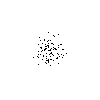
\includegraphics[keepaspectratio]{plots/4.png}}

\pandocbounded{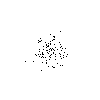
\includegraphics[keepaspectratio]{plots/5.png}}
\caption{Every 200th step throughout the simulation}\label{vis}
\end{figure}

For more complex example, consider evolutionary neural network
implementation {[}kaikalii\_evonet\_github{]} made by the creator of
Uiua, which demonstrates Uiua's potential for implementing advanced
ALife techniques.

\textsc{Conclusion}

The particle swarm simulation demonstrates Uiua's capabilities for ALife
research. By leveraging Uiua's array operations and functional
programming paradigms, researchers can create efficient and expressive
simulations of bio-like systems. The concise syntax and stack-based
approach enable rapid prototyping and iteration, facilitating hypothesis
testing and model refinement. By adopting Uiua, ALife researchers can
streamline their workflows, reduce boilerplate code, and focus more on
the scientific challenges at hand.
